%!TEX root = ./template-skripsi.tex
%-------------------------------------------------------------------------------
%                            BAB III
%               			PEMBAHASAN
%-------------------------------------------------------------------------------

\chapter{DESAIN MODEL}

\section{Tahapan Penelitian}

Berikut merupakan \emph{flowchart} dari tahapan penelitian \emph{Automatic Tagging} dengan menggunakan algoritma \emph{Bipartite Graph Partition} dan \emph{Two Way Poisson Mixture Model}.

\begin{figure}[H]
    \centering
    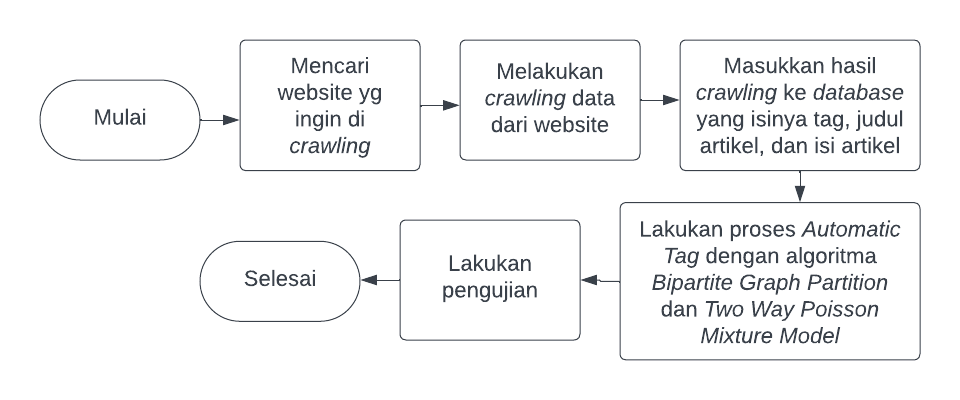
\includegraphics[width=1\textwidth]{gambar/Tahapan penelitian.png}
    \caption{Flowchart alur penelitian}
    \label{gambar:tahapan_penelitian}
\end{figure}

Mencari salah satu situs yang ingin di-\emph{crawling} terlebih dahulu. Kemudian, lakukan \emph{crawling} data dari situs tersebut menggunakan \emph{crawler} dari penelitian \cite{khatulistiwa_2022_searchengine}. Hasil \emph{crawling} tersebut dimasukkan ke dalam \emph{database}.

Kemudian, data tersebut diolah menggunakan algoritma \emph{Bipartite Graph Partition} dan \emph{Two Way Poisson Mixture Model} untuk melatih program supaya bisa memprediksi \emph{tag} yang diinginkan. Setelah itu, lakukan pengujian terhadap \emph{tag} yang telah dihasilkan.

% \section{Desain \textit{Automatic Tag }} 

% Pada proses pembuatan algoritma untuk pembuatan \textit{automatic tag}, penulis menggunakan algoritma \textit{Real Time Automatic Tag Recommendation}. 

% \textit{Real Time Automatic Tag Recommendation} berdasarkan algoritma yang dikembangkan oleh \citep{song2008autotag} adalah suatu sistem untuk merekomendasikan suatu \textit{tag-tag} untuk dokumen-dokumen yang di mana sistem ini memerlukan data latih. 

% Secara garis besar, algoritma ini memiliki dua tahap besar yaitu \textit{offline computation} atau tahap \textit{training data} dan \textit{online recommendation} atau tahap \textit{testing data}. 

% \textit{Offline computation} merupakan tahapan untuk mempelajari data-data dari kumpulan dokumen-dokumen ($D$), tag-tag ($T$), serta kata-kata ($S$) yang telah diberikan. Nantinya, data-data tersebut akan dibentuk ke dalam klaster-klaster ($K$) melalui algoritma \textit{Spectral Recursive Embedding} (\textit{SRE}). Selanjutnya, data-data yang telah diklaster, nantinya akan melakukan perangkingan terhadap suatu \textit{tag}. Selanjutnya, tahap untuk membuat \textit{Two Way Poisson Mixture Model}.

% Tahapan \textit{Online Recommendation} merupakan tahapan di mana suatu dokumen yang baru akan diberikan \textit{tag-tag} sesuai dengan klaster yang nantinya dokumen baru ini akan tempatkan.

% Tahapan \textit{Online Recommendation} merupakan tahapan di mana suatu dokumen yang baru saja diinput dan bukan yang diinput pada tahap \textit{Offline Computation} akan diberikan \textit{tag-tag} sesuai dengan klaster yang nantinya dokumen baru ini akan tempatkan.

\section{Algoritma \emph{Automatic Tag}}

Berikut adalah algoritma dari \textit{Online Tag Recommendation}

\begin{algorithm} [H]
\caption{Online Tag Recommendation \citep*{song2008autotag}}\label{alg:online_tag_recommendation_2}
\label{algoritma:automatic_tag}
\begin{algorithmic}
\State 1: \textbf{Input} $(\mathcal{D}, S, T), K, M, L$ \\
$\quad$ Kumpulan dokumen: $\mathcal{D}=\left\{\mathcal{D}_{1}, \ldots, \mathcal{D}_{m}\right\}$ \\
$\quad$ \textit{Word vocabulary}: $S=\left\{S_{1}, \ldots, S_{k}\right\}$ \\
$\quad$ \textit{Tag vocabulary}: $T=\left\{T_{1}, \ldots, T_{n}\right\}$ \\
$\quad$ banyaknya klaster: $K \in \mathbb{R}$ \\
$\quad$ banyaknya komponen-komponen: $M \in \mathbb{R}$ \\
$\quad$ banyaknya klaster-klaster kata: $ L \in \mathbb{R} $ \\
\textit{\textbf{Offline Computation}} \\
2: Menunjukkan bobot terdekat matriks W seperti persamaan (\ref{w_ab}) \\
3: Normalisasi $W$ menggunakan \textit{Normalized Laplacian} persamaan (\ref{normalize_laplacian}) \\
4: Komputasi \textit{low rank approximation matrix} menggunakan Lanczos: \\
$\quad \tilde{W} \simeq L(W)=Q_{k} T_{k} Q_{k}^{T}$ \\
5: Partisi $\tilde{W}$ ke dalam klaster K menggunakan SRE, 
$\quad \tilde{W}=\left\{\tilde{W}_{1}, \ldots, \tilde{W}_{K}\right\}$ \\
6: Tandai label ke dalam setiap dokumen $\mathcal{D}_{j}, j \in\{1, \ldots m\}$ \\
$\quad C\left(\mathcal{D}_{j}\right) \in\{1, \ldots, K\}$ \\
7: Hitung \textit{node rank} $Rank(T)$ untuk setiap tag $T_{i, k}$ di dalam klaster \\
$k, i \in\{1, \ldots, n\}, k\{1, \ldots, K\} \quad$ persamaan (\ref{rank_i}) \\
8: Buat \textit{Poisson Mixture Model} untuk $(\tilde{B}, C(\mathcal{D}))$ dengan $M$ komponen-komponen dan $L$ klaster kata-kata, di mana $\tilde{B}$ denotasi matriks inter-relationship pada suatu dokumen-dokumen dan kata-kata di dalam $\tilde{W}$ persamaan (\ref{w_ab})\\
\textit{\textbf{Online Recommendation}} \\
9: Untuk setiap dokumen tes $\mathbb{Y}$, kalkulasikan posterior probabilitas \\
$P(C=k \mid D=\mathbb{Y})$ di dalam setiap klaster $k$, dan denotasi membership pada $\mathbb{Y}$ sebagai $C(\mathbb{Y})=\{c(\mathbb{Y}, 1), \ldots, c(\mathbb{Y}, K)\}$ persamaan (\ref{bayes_rules}) \\
10: Tag rekomendasi berdasarkan perangkingan pada tag, yaitu \textit{joint probability} pada tag-tag $T$ dan dokumen $Y$, $R(T, \mathbb{Y})$ persamaan (\ref{rank_tag}) \\
\end{algorithmic}
\end{algorithm}

\section{Flowchart Automatic Tag}
\begin{figure}[H]
    \centering
    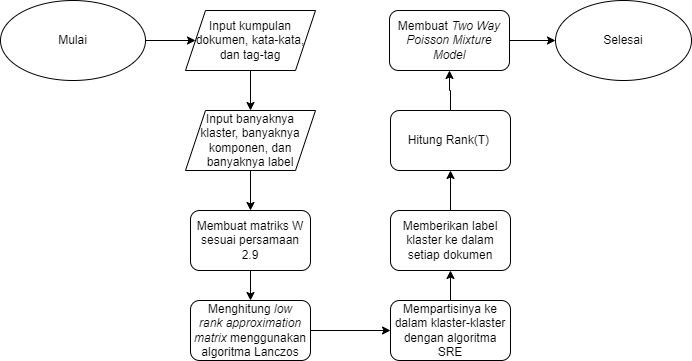
\includegraphics[width=1\textwidth]{gambar/Tag Flowchart.drawio.png}
    \caption{Diagram alir untuk tahap \textit{offline computation}}
    \label{gambar:flowchart_automatic_tag}
\end{figure}

\begin{figure}[H]
    \centering
    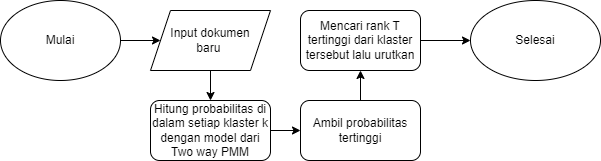
\includegraphics[width=1\textwidth]{gambar/Online Recommendation Flowchart.png}
    \caption{Melakukan \textit{online recommendation} berdasarkan hasil data training}
    \label{gambar:online_recomendation_tag}
\end{figure}

\section{Alat dan Bahan Penelitian}

Dalam penelitian ini, setidaknya ada perangkat keras sebagai berikut.

\begin{enumerate}
    \item Laptop dengan prosesor Intel Core i5 8th Gen \textit{series} dan \textit{RAM} 16 \textit{GB}.
    \item Koneksi berbasis Wi-Fi dan berbasis kuota internet dari ponsel pintar.
\end{enumerate}

Perangkat lunaknya sebagai berikut.

\begin{enumerate}
    \item Windows 10 64 bit OS.
    \item Visual Studio Code sebagai \textit{Code Editor}.
    \item Python 3 untuk menjalankan program Python.
    \item Sumber data berasal dari \textit{Thehill.com} .
\end{enumerate}

\section{Tahapan Penelitian Automatic Tag}

Setidaknya terdapat 10 tahapan yang perlu dijalankan agar \textit{automatic tag} ini akan berjalan dengan baik yaitu

\subsection{Penginputan}

Pada tahap ini, akan ditentukan enam komponen atau inputan yang diperlukan adalah dokumen ($D$), \textit{word vocabulary} ($S$), \textit{Tag vocabulary} ($T$), banyaknya klaster ($K$), banyaknya komponen-komponen ($M$), dan banyaknya klaster-klaster kata ($L$).

Untuk dokumen ($D$) yang diinput, berasal dari data hasil \textit{crawling} dengan menggunakan \textit{crawler} milik Lazuardy Khatulistiwa berjudul Perancangan Arsitektur \textit{Search Engine} dengan Mengintegrasikan \textit{Web Crawler}, Algoritma \textit{Page Ranking}, dan \textit{Document Ranking}.

Untuk \textit{word vocabulary} ($S$), kata-kata yang diinput merupakan kata-kata yang berasal dari dokumen hasil \textit{crawling}.

Pada \textit{tag vocabulary ($T$)}, \textit{tag} yang didapat berasal dari dokumen \textit{tag} hasil \textit{crawling}. 

Pada banyaknya klaster ($K$), digunakan untuk menentukan berapa klaster yang ingin dibuat saat menjalankan algoritma \textit{SRE}. Banyaknya klaster ini ditentukan sesuai dengan keinginan sang pengguna.

Banyaknya komponen-komponen ($M$), biasanya $M$ ini akan digunakan pada algoritma \textit{Two Way Poisson Mixture Model}.

Terakhir adalah banyaknya klaster kata ($L$) untuk melakukan pelabelan ($L$). Variabel ini akan digunakan pada algoritma \textit{Two Way Poisson Mixture Model}.

\subsection{Menentukan Matriks W}
Untuk matriks $W$ akan terdiri dari beragam matriks yaitu matriks $A$, matriks $A^T$, matriks $B$, dan matriks $B^T$.

Untuk matriks $A$, terbuat dari relasi antara \textit{tag vocabulary} dengan dokumen, sedangkan untuk matriks $B$ diperoleh dari relasi antara dokumen dengan \textit{word vocabulary}.

Untuk membuat matriks $W$ akan menggunakan persamaan (\ref{w_ab}). Untuk contohnya, akan mengambil gambar berikut.

\begin{figure}[h]
    \centering
    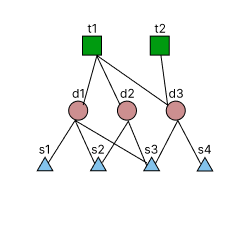
\includegraphics[width=0.75\textwidth]{gambar/Bipartite Graph Simple.png}
    \caption{Contoh simpel dua \textit{bipartite graph}}
    \label{gambar:simple_bipartite_graph}
\end{figure}

Relasi antara $t$ (\textit{tag}) dengan $d$ (\textit{document}) akan membentuk matriks $A$ dan $A^T$ sebagai berikut.

\begin{equation}
    A = \begin{pmatrix}
1 & 1 & 1 \\
0 & 0 & 1 \\
\end{pmatrix}
\end{equation}

\begin{equation}
    A^T = \begin{pmatrix}
1 & 0 \\
1 & 0 \\
1 & 1 \\
\end{pmatrix}
\end{equation}

Selanjutnya, mencari relasi antara $D$ (\textit{document}) dengan $S$ (\textit{words}) agar membentuk \textbf{matriks $B$} sebagai berikut.

\begin{equation}
    B = \begin{pmatrix}
1 & 1 & 1 & 0 \\
0 & 1 & 1 & 0 \\
0 & 0 & 1 & 1 \\
\end{pmatrix}
\end{equation}

\begin{equation}
    B^T = \begin{pmatrix}
1 & 0 & 0 \\
1 & 1 & 0 \\
1 & 1 & 1 \\
0 & 0 & 1 \\
\end{pmatrix}
\end{equation}

Selanjutnya, adanya penggabungan yang nantinya membentuk \textbf{matriks $W$} sebagai berikut

\begin{equation*}
    W = \begin{pmatrix}
0 & A & 0\\
A^T & 0 & B\\
0 & B^T & 0
\end{pmatrix}
\end{equation*}

Nantinya, matriks $A$ dan matriks $B$ ditempatkan ke dalam matriks $W$. Angka 0 di atas merupakan matriks 0 yang isinya menyesuaikan baris dan kolom matriks sekitarnya.

\begin{equation}
    W = \begin{pmatrix}
0 & 0 & 1 & 1 & 1 & 0 & 0 & 0 & 0 \\
0 & 0 & 0 & 0 & 1 & 0 & 0 & 0 & 0 \\
1 & 0 & 0 & 0 & 0 & 1 & 1 & 1 & 0 \\
1 & 0 & 0 & 0 & 0 & 0 & 1 & 1 & 0 \\
1 & 1 & 0 & 0 & 0 & 0 & 0 & 1 & 1 \\
0 & 0 & 1 & 0 & 0 & 0 & 0 & 0 & 0 \\
0 & 0 & 1 & 1 & 0 & 0 & 0 & 0 & 0 \\
0 & 0 & 1 & 1 & 1 & 0 & 0 & 0 & 0 \\
0 & 0 & 0 & 0 & 1 & 0 & 0 & 0 & 0 \\
\end{pmatrix}
\end{equation}

% \subsection{Normalisasi $W$ menggunakan \textit{Normalized Laplacian}}

% Pada persamaan normalisasi Laplacian, diperlukan dua jenis matriks yaitu matriks $W$ dan matriks $D$. Untuk mengisi matriks diagonal $D$ diperlukan mengisi $D_{ii}$ terlebih dahulu. Untuk mendapatkan $D_{ii}$ memerlukan $d_i$ yang berasal dari $d_{i}=\sum w_{i j}$ . $w_{ij}$ didapat dari matriks $W$.

% \begin{equation}
%     D = \begin{pmatrix}
% 3 & 0 & 0 & 0 & 0 & 0 & 0 & 0 & 0\\
% 0 & 1 & 0 & 0 & 0 & 0 & 0 & 0 & 0\\
% 0 & 0 & 4 & 0 & 0 & 0 & 0 & 0 & 0\\
% 0 & 0 & 0 & 3 & 0 & 0 & 0 & 0 & 0\\
% 0 & 0 & 0 & 0 & 4 & 0 & 0 & 0 & 0\\
% 0 & 0 & 0 & 0 & 0 & 1 & 0 & 0 & 0\\
% 0 & 0 & 0 & 0 & 0 & 0 & 2 & 0 & 0\\
% 0 & 0 & 0 & 0 & 0 & 0 & 0 & 3 & 0\\
% 0 & 0 & 0 & 0 & 0 & 0 & 0 & 0 & 1\\
% \end{pmatrix}
% \end{equation}

% Setelah mendapatkan $D$ dan $W$, lalu masukkan ke persamaan normalisasi Laplacian hingga membentuk $L(W)$. $L(W)$ yang dicontohkan di sini hasil dari pembulatan agar lebih mudah terbaca, tetapi dalam kasus nyatanya, tidak ada pembulatan.

% \begin{equation}
%     L(W) = \begin{pmatrix}
% 0 & 0 & 0.29 & 0.33 & 0.29 & 0 & 0 & 0 & 0\\
% 0 & 0 & 0 & 0 & 0.5 & 0 & 0 & 0 & 0\\
% 0.29 & 0 & 0 & 0 & 0 & 0.5 & 0.35 & 0.29 & 0\\
% 0.33 & 0 & 0 & 0 & 0 & 0 & 0.41 & 0.33 & 0\\
% 0.29 & 0.5 & 0 & 0 & 0 & 0 & 0 & 0.29 & 0.5 \\
% 0 & 0 & 0.5 & 0 & 0 & 0 & 0 & 0 & 0\\
% 0 & 0 & 0.35 & 0.41 & 0 & 0 & 0 & 0 & 0\\
% 0 & 0 & 0.29 & 0.33 & 0.29 & 0 & 0 & 0 & 0\\
% 0 & 0 & 0 & 0 & 0.5 & 0 & 0 & 0 & 0 \\
% \end{pmatrix}
% \end{equation}

\subsection{Menghitung \textit{Low Rank Approximation Matrix} menggunakan algoritma Lanczos}

Pada algoritma Lanczos yang terdapat di (\cite{golub_matrix_computation_3_edition}), ada beberapa inputan agar prosesnya bisa berjalan yaitu $\beta_0$, $q_0$, $b$, dan $q_1$. Berikut adalah beberapa inputannya.

\begin{equation*}
    \beta_0 = 0
\end{equation*}
\begin{equation*}
    q_0 = 0
\end{equation*}
\begin{equation*}
    b = arbitrary
\end{equation*}

Karena $b$ adalah \textit{arbitrary} yang memiliki makna bahwa nilai yang diinput itu bebas. Oleh karena itu, $b$ dibuat menjadi

\begin{equation*}
    b = \begin{pmatrix}
        1 & 1 & 1 & 1 & 1 & 1 & 1 & 1 & 1
    \end{pmatrix}
\end{equation*}

Selanjutnya nilai $q_1$ adalah

\begin{equation*}
    q_1 = b/||b|| = \begin{pmatrix}
        0.33 & 0.33 & 0.33 & 0.33 & 0.33 & 0.33 & 0.33 & 0.33 & 0.33 
    \end{pmatrix}
\end{equation*}

\begin{equation}
    \quad \hat{W} \simeq L(W)=Q_{k} T_{k} Q_{k}^{T}
\end{equation}

Karena persamaan ini, hasil dari $L(W)$ juga bisa dicari dengan menggunakan $\hat{W}$. Selain itu, algoritma Lanczos dinilai lebih efisien untuk data yang banyak dibandingkan menggunakan normalisasi Laplacian.  Untuk mencari $Q_k$ dan $T_k$, perlu menggunakan iterasi Lanczos. 

Untuk matriks $T_k$ memiliki format sebagai berikut

\begin{equation*}
T_{k}=\left[\begin{array}{ccccc}
\alpha_{1} & \beta_{1} & & & \\
\beta_{1} & \alpha_{2} & \beta_{2} & & \\
& \beta_{2} & \alpha_{3} & \ddots & \\
& & \ddots & \ddots & \beta_{k-1} \\
& & & \beta_{k-1} & \alpha_{k}
\end{array}\right] .
\end{equation*}

Dalam matriks di atas, diperlukan pencarian nilai $\alpha$ dan $\beta$ agar bisa melengkapi hasil $T_k$.

Untuk matriks $Q_k$ didapat dari
\begin{equation*}
    Q_k = \begin{pmatrix}
q_1 &|& q_2 &|& \dots &|& q_k
\end{pmatrix}
\end{equation*}

$q_1$ adalah matriks kolom yang ke-1. $q_2$ adalah matriks kolom yang ke-2. $q_k$ adalah matriks kolom yang ke-k. $q_1$ sampai $q_k$ akan didapat melalui iterasi Lanczos sebagai berikut.

Pada algoritma di bawah, asumsikan bahwa $n = k$ dan $A = W$.

\begin{algorithm}[H]
    \caption{\textit{Lanczos Iteration} \citep*{golub_matrix_computation_3_edition}}\label{alg:lanczos}
    \begin{algorithmic}
        \Require $\beta_0 = 0$, $q_0 = 0$, $b = arbitrary$, $q_1 = b/||b||$
        \While{$n = 1,2,3,.. $}
        \State $v = Aq_n$
        \State $\alpha_n = q_n^Tv $
        \State $v = v - \beta_{n-1} q_{n-1} - \alpha_n q_n $
        \State $\beta_n = ||v|| $ 
        \State $q_{n+1} = v/\beta_n $
        \EndWhile
    \end{algorithmic}
\end{algorithm}

\subsection{Melakukan partisi $\hat{W}$ ke dalam klaster K menggunakan \textit{SRE}}

Untuk membuat algoritma \textit{SRE} berdasarkan \cite{zha2001bgp}, ada lima langkah yang diperlukan.

Pertama adalah menghitung $D_X$ dan $D_Y$ dan membentuk matriks $\hat{W} = D_X^{-1/2}WD_Y^{-1/2}$. Pada langkah ini, matriks $\hat{W}$ telah dibuat dengan menggunakan algoritma Lanczos atau \textit{normalized Laplacian}. Alasannya adalah pola untuk mendapatkan $\hat{W}$ yang mirip.

Langkah kedua ialah mencari vektor terluas kedua singular kiri dan singular kanan dengan menggunakan \emph{Singular Vector Decomposition} (\emph{SVD}) .

Dalam algoritma \textit{SRE}, langkah ketiga adalah mencari titik potong yaitu $c_x$ dan $c_y$ untuk $x = D_X^{-1/2}\hat{x}$ dan $y = D_Y^{-1/2}\hat{y}$. Untuk mencari keduanya, strategi tersimpelnya adalah dengan memasang $c_x = 0$ dan $c_y = 0$. 

Langkah keempatnya membentuk suatu partisi dengan $A = \{i | x_i \geq c_x\}$ dan $A^C = \{i | x_i < c_x\}$ untuk \textit{vertex} $X$ dan $B = \{i | y_j \geq c_y\}$ dan $B^C = \{j | y_j < c_x\}$ untuk \textit{vertex} $Y$.

Langkah kelima adalah mengulangi partisi pada \textit{sub graph} $G(A,B)$ dan $G(A^c,B^c)$ jika diperlukan.

Berikut ini adalah algoritma \textit{Spectral Recursive Embedding} atau \textit{SRE} dari \citep*{zha2001bgp}

\begin{algorithm}[H]
\caption{\textit{\textit{Spectral Recursive Embedding (SRE)}} \citep*{zha2001bgp}}\label{alg:sre}
\begin{algorithmic}

\State Diberikan \textit{weighted bipartite graph} $G = (X, Y, E)$ dengan bobot garis matriks $W$ \\

1. Komputasi $D_x$ dan $D_y$ dan bentuk \textit{scaled weight matrix} $\hat(W) = D_x^{-1/2} W D_y^{-1/2}$ \\

2. Hitung singular vektor terluas kiri dan kanan kedua dari vektor $\hat{W}$, $\hat{x}$, dan $\hat{y}$ \\

3. Temukan titik potong $c_x$ dan $c_y$ untuk $x = D_X^{-1/2} \hat{x}$ dan $y = D_Y^{-1/2} \hat{y}$, secara berulang. \\

4. Bentuk partisi $A = \{i | x_i \geq c_x\}$ dan $A^c = \{i | x_i < c_x\}$ untuk verteks set X, dan  $B = \{j | y_j \geq c_y\}$ dan $B^c = \{j | y_j < c_y\}$ untuk verteks set Y. \\

5. Lakukan partisi secara rekursif untuk \textit{sub-graphs} $G(A, B)$ dan $G(A^c, B^c)$ \\

\end{algorithmic}
\end{algorithm}

\subsection{Melakukan pelabelan setiap dokumen}

Selanjutnya adalah memberikan label kepada setiap dokumen yang ada sesuai pembagian klasternya. Misalnya, terdapat 4 dokumen yaitu $D_1$, $D_2$, $D_3$, dan $D_4$ dan ada 2 klaster sesuai jumlah $K$. Nantinya, dokumen tersebut dimasukkan ke dalam klaster sesuai dengan hasil partisi $\hat{W}$ sesuai dengan banyaknya klaster yang dibentuk.

\subsection{Menghitung \textit{Node Rank} Rank(T) untuk Setiap Tag}

Cara menghitung Rank(T) untuk setiap tag $T_i$ di dalam klaster $k$ dengan menggunakan persamaan (\ref{n_precision}), persamaan (\ref{n_recall}), dan persamaan (\ref{rank_i}).

Untuk persamaan (\ref{n_precision}) adalah menghitung \textit{N-Precision} $np_i$. Untuk mencari $np_i$, diharuskan menghitung total seluruh bobot \textit{edges} dari \textit{node} $i$ di dalam klaster yang sama, lalu hasilnya dibagi dengan total dari seluruh bobot pada \textit{edges} di klaster tersebut. Semakin besar nilai $np_i$-nya, semakin penting keberadaan \textit{tag} di dalam klaster tersebut.

Untuk persamaan (\ref{n_recall}) adalah menghitung \textit{N-recall}. $|E_i|$ didapat dari banyaknya garis yang terhubung ke Tag i $T_i$ baik itu di dalam klaster maupun di luar klaster. Lalu, hasilnya dibagi dengan banyaknya garis  yang terhubung dengan $T_i$ yang di luar klaster.

Setelah berhasil menghitung $np_i$ dan $nr_i$, $Rank_i$ dapat dihitung dengan $exp(\frac{-1}{r(i)^2})$ untuk $r(i) = np_i * log(nr_i)$ dengan syarat $r(i)$ tidak boleh sama dengan 0. Jika $r(i) = 0$, $Rank_i$ hasilnya adalah 0 berdasarkan persamaan (\ref{rank_i}).

\subsection{Membuat Two Way Poisson Mixture Model}

Untuk membuat salah satu komponen dari \textit{Two Way Poisson Mixture Model}, diperlukan persamaan (\ref{poisson_mixture_model_2}). Salah satu komponen dari persaman tersebut adalah $\phi_m$ yang didapat dari persamaan (\ref{update_parameter_lambda}). 

Untuk $II(F(m) = k)$ adalah suatu \textit{indicator function}. Jika komponen m milik klaster k, berarti bernilai 1. Dalam kondisi sebaliknya, bernilai 0.

Untuk mengisi $t$ pada persamaan (\ref{update_parameter_pi}), inisialisasi $t = 0$ (\cite{jia_2004_two_way_poisson_model}). Kemudian, saat mencari persamaan (\ref{update_parameter_pi}), terdapat komponen $p_{i,m}$ yang perlu dicari terlebih dahulu dengan menggunakan persamaan (\ref{poisson_mixture_model_2}). 

Pada $p_{i,m}$ terdapat komponen $\phi^{(t)}_m$. Kemudian, $d(i,j)$ didapat dari berapa banyaknya kata $j$ di dalam dokumen $i $. Hal ini ada hubungannya dengan matriks $B$ dari persamaan (\ref{w_ab}). Mencari $\theta$ dapat dicari dengan cara $\theta(d_j | \lambda_{j,m}) = e^{- \lambda_{j,m}}\lambda_{j,m}^{d_j}/d_j!$. Untuk $p$, ia adalah \textit{dimension}. Selain itu, $IIC(i)$ untuk mengecek apakah kata $i$ ada di klaster tersebut. 

Selain itu, di persamaan (\ref{poisson_mixture_model_2}) terdapat komponen $\Tilde{\lambda}_{m,l}$ yang bisa ditemukan di persamaan (\ref{update_parameter_lambda}). Pada variabel $|d(i,j)|$ dapat dicari dengan menentukan apakah $j$ ada di label $l$.

\subsection{Rekomendasi Tag Untuk Dokumen Baru}

Lakukan melalui persamaan (\ref{bayes_rules}) lalu untuk mencari $\frac{P(D = d_t|C = k) P(C=k)}{P(D=d_t)}$ bisa ditemukan dengan persamaan (\ref{poisson_mixture_model_2}). Lalu, masukan dokumen yang baru ke dalam suatu klaster yang memiliki probabilitas terbesar.

\subsection{Rekomendasi Tag Berdasarkan Ranks Tag}

Setelah melakukan perhitungan $P(C = k|D = Y)$, langkah berikutnya adalah merekomendasikan \textit{tag-tag} berdasarkan klaster dari dokumen tersebut. Cara melakukannya adalah dengan menggunakan persamaan (\ref{rank_tag}) pada setiap \textit{tag} yang ada di klaster tersebut. Kemudian, lakukan pengurutan $R(T_i, d_t)$ dari yang terbesar ke yang terkecil.

% \section{Skenario Eksperimen}

% Berikut adalah skenario eksperimen untuk \textit{Automatic Tag Recommendation}

% \begin{enumerate}
%     \item \textit{Crawling} data baru dari web yang artikelnya ada \textit{tagging}-nya.
%     \item Dokumentasikan sumber datanya.
%     \item Mencari data sampel dengan minimal 2000 artikel dokumen HTML yang berasal dari satu domain yang sama.
%     \item Hitung jumlah \textit{tag} yg unik dari dataset tersebut.
%     \item Hitung jumlah tag per dokumen dengan statistiknya.
%     \item Pergunakan 1000 dokumen sebagai \textit{offline learning} atau untuk data \textit{training}.
%     \item Pastikan antara \textit{learning} dengan \textit{prediction} tidak ada \textit{tag} yang terlewat.
%     \item Lakukan \textit{offline learning} dengan menset jumlah klaster.
%     \item Lakukan pengujian secara otomatis pada seluruh dokumen yang diuji.
% \end{enumerate}

\section{Skenario Pengujian}

Berikut adalah skenario pengujian untuk \textit{Automatic Tag Recommendation} dengan Algoritma \textit{Bipartite Graph Partition} dan \textit{Two Way Poisson Mixture Model}.

\begin{enumerate}
    \item Sumber data yang didapat dari hasil \textit{crawling} dibagi menjadi dua bagian yaitu untuk data latih dan data uji.
    \item Setelah seluruh proses algoritmanya berjalan, data uji mulai dimasukkan.
    \item Program akan memberikan beberapa prediksi \textit{tag} pada data uji.
    \item Kemudian, menghitung banyaknya \textit{tag} yang cocok dengan data uji. 
\end{enumerate}
%Now I think about this the key question isn't about query but how to measure the successfulness of BFS and Modified similarity crawler.
%To proven this question, I think your crawler should be run in two different situation:
%a. Crawler which run for a site only
%b. Crawler which run for a site, but continue crawling until stop. 
%You can return page map graph for the first situation. And you can return the same thing on the second situation but instead of page map you return site map.